%%% =====================================================================
%%% figset_E.tex  --  TikZ figure set E of the QCD factorization monograph
%%%   (agent figE, local style prefix "fe"):
%%%   Ch24 `front' (FIGURES_INDEX_v2 Sec. 4.4: Gordan alternative, regions and
%%%   Newton polytopes, endpoint factorization, Yukawa-model MSbar pdf;
%%%   optional: super-leading logarithms, DPS double counting),
%%%   App M (Sec. 4.5 and Sec. 3: dependency graph, BPHZ forests and normal
%%%   products, handbag as AB part vs reduced graph, Euclidean vs forward
%%%   kinematics), App N (Sec. 4.6: one-loop triangle regions and remainder;
%%%   optional: pairing decomposition on the nine-region poset).
%%% 13 figures: 10 required + 3 optional (front-sll, front-dps-double-counting,
%%%   appN-chain-pairing).  External label referenced: fig:method-hasse (Ch9).
%%%
%%% Requirements: preamble_fact.tex (ctexbook, XeLaTeX), which loads tikz with
%%%   decorations.pathmorphing, decorations.markings, arrows.meta, calc,
%%%   positioning, shapes.geometric, patterns, backgrounds, fit, pgfplots
%%%   (compat=1.17) and contains the style blocks STYLES / STYLES-EXT; plus the
%%%   preamble macros \ii \dd \ee \MSbar \kT \Real, \cref (cleveref), \cite,
%%%   dvipsnames colours (OliveGreen, RoyalBlue), amssymb (\curvearrowleft,
%%%   \varnothing) and booktabs (table in fig:appN-chain-pairing).  No package
%%%   or library beyond the preamble is used (no decorations.pathreplacing:
%%%   the braces in fig:front-sll are drawn by hand).
%%% Every extra style is declared in the options of its tikzpicture (hence
%%% local to that picture) and carries the prefix "fe"; the few helper macros
%%% (\fegl, \fest, \fehw, \feR, \feM, \feT) are defined inside a tikzpicture and
%%% are therefore local to it as well.
%%% Numbers and closed forms: VERIFIED_FORMULAS_v2 (IDs quoted in the
%%% captions); pgfplots curves either from the VF formula as a pgfplots
%%% expression or from inline coordinate tables computed from it (the
%%% generating script is quoted in a comment inside the block).
%%%
%%% Drawing conventions used throughout this set (as in figures1-3)
%%%   * solid line with arrow = quark; the arrow is the fermion-number flow;
%%%   * thin separate arrow with label (styles mom/mom') = momentum flow;
%%%   * double line with arrow = Wilson (eikonal) line;
%%%   * blob colours as in fd_styles_ext: grey = hard, blue = collinear to
%%%     n_A (or n_1), orange = collinear to n_B (or n_2), green = soft,
%%%     light grey = hadron / non-perturbative;
%%%   * dashed rounded box (style region) = subgraph or momentum region;
%%%   * dependency graphs: fills by rigour tag (as \tagR \tagA ...),
%%%     dashed border = R_cond statement, orange dashed box = numbered
%%%     assumption (as the App P generator, FIGURES_INDEX_v2 Sec. 4.9).
%%% =====================================================================

%%% BEGIN fig:front-gordan
\begin{figure}[htbp]
\centering
% Data: (a) D1=(2,0), D2=(1,2) (ex:front-gordan-2d), D3=(2.6,1.6) on the far side of the
% line D1D2; min-norm point of conv{D_j}: w=(8/5,4/5), |w|^2=16/5=D1.w=D2.w, D3.w=5.44;
% good cone {v: D_j.v>0} = directions between -26.57 deg (perp. to D2) and 90 deg (perp. to D1).
% (b) D3=(-1,-1): 1*D1+2*D2+4*D3=0 (closed polygon drawn at scale 0.4).
\begin{tikzpicture}[fd,
  fe vec/.style={draw,line width=0.9pt,-{Stealth[length=6pt,width=4.6pt]}},
  fe hull/.style={draw=gray!65,fill=gray!22,line width=0.6pt,line join=round},
  fe cone/.style={fill=green!9,draw=none},
  fe ray/.style={draw=green!45!black,line width=0.6pt,dash pattern=on 3pt off 2pt},
  fe wpt/.style={circle,fill=red!65!black,draw=none,inner sep=0pt,minimum size=4.6pt},
  fe lam/.style={draw=blue!60!black,line width=0.9pt,-{Stealth[length=6pt,width=4.6pt]}},
  fe lab/.style={font=\footnotesize}]
  % ======================= (a) good direction =======================
  \begin{scope}
    \fill[fe cone] (0,0) -- (-26.565:2.95) arc[start angle=-26.565,end angle=90,radius=2.95] -- cycle;
    \draw[fe ray] (0,0) -- (90:2.95);
    \draw[fe ray] (0,0) -- (-26.565:2.95);
    \draw[lcaxis,gray!55] (-1.15,0) -- (3.35,0);
    \draw[lcaxis,gray!55] (0,-1.75) -- (0,3.3);
    % supporting line v.w = |w|^2 through D1, D2
    \draw[gray!60!black,densely dotted,line width=0.6pt] ($(2,0)!-0.45!(1,2)$) -- ($(2,0)!1.32!(1,2)$);
    \draw[fe hull] (2,0) -- (1,2) -- (2.6,1.6) -- cycle;
    \draw[fe vec] (0,0) -- (2,0);
    \draw[fe vec] (0,0) -- (1,2);
    \draw[fe vec] (0,0) -- (2.6,1.6);
    \draw[red!65!black,line width=0.7pt,dash pattern=on 2.5pt off 1.8pt] (0,0) -- (1.6,0.8);
    % right-angle mark at w on the D1 side (face direction (1,-2)/sqrt5, normal (2,1)/sqrt5),
    % away from the arrow D3 which passes just above w
    \draw[red!65!black,line width=0.5pt] ($(1.6,0.8)+(0.0894,-0.1789)$) -- ++(-0.1789,-0.0894) -- ++(-0.0894,0.1789);
    \node[fe wpt] at (1.6,0.8) {};
    \node[anchor=north east,inner sep=1.5pt] at (2.02,-0.03) {$D_1$};
    \node[anchor=east,inner sep=2pt] at (0.98,2.05) {$D_2$};
    \node[anchor=west,inner sep=2pt] at (2.62,1.62) {$D_3$};
    \node[inner sep=1pt,text=red!60!black] at (1.27,0.42) {$w$};
    \node[fill=white,fill opacity=0.85,text opacity=1,inner sep=1pt] at (0,0) {};
    \node[anchor=north east,inner sep=1.5pt] at (0,0) {$0$};
    \node[fe lab,text=green!35!black,anchor=south,align=center] at (1.5,2.82) {好方向锥 $\{v:D_j\cdot v>0\}$};
    \node[fe lab,text=gray!40!black,anchor=north west] at (2.38,-0.62) {$v\cdot w=|w|^2$};
    \node at (1.05,-2.25) {(a)\ $D_j\cdot w\ge|w|^2$：好方向};
  \end{scope}
  % ======================= (b) Landau point =======================
  \begin{scope}[xshift=7.1cm]
    \draw[lcaxis,gray!55] (-1.75,0) -- (2.75,0);
    \draw[lcaxis,gray!55] (0,-1.75) -- (0,3.3);
    \draw[fe hull] (2,0) -- (1,2) -- (-1,-1) -- cycle;
    \draw[fe vec] (0,0) -- (2,0);
    \draw[fe vec] (0,0) -- (1,2);
    \draw[fe vec] (0,0) -- (-1,-1);
    \node[circle,fill=black,draw=none,inner sep=0pt,minimum size=3.6pt] at (0,0) {};
    \node[anchor=north west,inner sep=1.5pt] at (1.98,-0.03) {$D_1$};
    \node[anchor=east,inner sep=2pt] at (0.98,2.05) {$D_2$};
    \node[anchor=north east,inner sep=1.5pt] at (-1,-1) {$D_3$};
    \node[anchor=south east,inner sep=1.5pt] at (-0.05,0.05) {$0$};
    % closed polygon of the weighted vectors (scale 0.4)
    \begin{scope}[shift={(2.85,0.55)},scale=0.4]
      \draw[fe lam] (0,0) -- (2,0);
      \draw[fe lam] (2,0) -- (4,4);
      \draw[fe lam] (4,4) -- (0,0);
      \node[fe lab,anchor=north,inner sep=2pt] at (1,0) {$\lambda_1D_1$};
      \node[fe lab,anchor=west,inner sep=2pt] at (3,2) {$\lambda_2D_2$};
      \node[fe lab,anchor=south east,inner sep=1pt] at (2,2.05) {$\lambda_3D_3$};
    \end{scope}
    \node[fe lab,align=center,anchor=north] at (3.6,-0.35) {$\lambda=(1,2,4)$\\[1pt]$\sum_j\lambda_jD_j=0$};
    \node at (1.25,-2.25) {(b)\ Landau 点：无好方向};
  \end{scope}
\end{tikzpicture}
\caption{Gordan 二择一定理（1873）\cite{Gordan1873}：对有限个对偶矢量 $D_j$，要么存在好方向 $v$（$D_j\cdot v>0$，可取凸包中范数最小的点 $w$，并有 $D_j\cdot w\ge|w|^2$），要么存在 Landau 点（$\lambda_j\ge0$ 不全为零、$\sum_j\lambda_jD_j=0$），二者恰有其一。
(a)~$D_1=(2,0)$、$D_2=(1,2)$ 与 $D_3$ 的凸包（灰）不含原点，最小范数点 $w=(\frac85,\frac45)$ 落在面 $D_1D_2$ 上（$D_1\cdot w=D_2\cdot w=|w|^2$），位于好方向锥（绿）之内；
(b)~换成 $D_3=(-1,-1)$ 后凸包含原点，$1\cdot D_1+2\cdot D_2+4\cdot D_3=0$（蓝色闭合折线），不存在好方向。
在 Collins\cite{Collins:2020euz}（2020，预印本）的符号条件下，积分围道在 $w_S$ 被钳住当且仅当存在 Landau 点（VF-FRO-1，VF-FRO-2）。}
\label{fig:front-gordan}
\end{figure}
%%% END fig:front-gordan

%%% BEGIN fig:front-regions-polytope
\begin{figure}[htbp]
\centering
% Schematic only (no data): a Newton polygon with lower chain S, C1, H, C2 (the adjacency
% S-C1-H-C2 is that of the four essential facets of the one-loop off-shell triangle;
% the 2D shape itself is not a projection of that polytope).
\begin{tikzpicture}[fd,x=0.56cm,y=0.56cm,
  fe poly/.style={draw=gray!60,fill=gray!10,line width=0.6pt,line join=round},
  fe pt/.style={circle,fill=black,draw=none,inner sep=0pt,minimum size=3.4pt},
  fe ipt/.style={circle,fill=gray!55,draw=none,inner sep=0pt,minimum size=3pt},
  fe facet/.style={line width=1.7pt,line cap=round},
  fe normal/.style={draw,line width=0.6pt,-{Stealth[length=4pt,width=3.4pt]}},
  fe sign/.style={circle,fill=white,line width=0.7pt,inner sep=0pt,minimum size=8.5pt,font=\scriptsize\bfseries},
  fe lab/.style={font=\footnotesize}]
  % ======================= (a) Euclidean type =======================
  \begin{scope}
    \draw[lcaxis] (-0.7,-0.7) -- (9.4,-0.7) node[below left=1pt,fe lab] {$x$ 的指数（投影）};
    \draw[lcaxis] (-0.7,-0.7) -- (-0.7,6.1) node[right=1pt,fe lab] {$t$ 的指数};
    \draw[fe poly] (0,3) -- (1,1) -- (3,0) -- (6,0) -- (8,1) -- (8,3) -- (6,5) -- (2,5) -- cycle;
    \draw[fe facet,green!45!black] (0,3) -- (1,1);
    \draw[fe facet,blue!60!black] (1,1) -- (3,0);
    \draw[fe facet,black!65] (3,0) -- (6,0);
    \draw[fe facet,orange!80!black] (6,0) -- (8,1);
    \foreach \p in {(0,3),(1,1),(3,0),(6,0),(8,1),(8,3),(6,5),(2,5),(4,0)} \node[fe pt] at \p {};
    \foreach \p in {(2,2),(3,3),(5,2),(6,3),(4,4),(2,4)} \node[fe ipt] at \p {};
    % inward normals of the lower facets (r_{n+1}>0)
    \draw[fe normal,green!45!black] (0.5,2) -- ++(0.894*1.3,0.447*1.3);
    \draw[fe normal,blue!60!black] (2,0.5) -- ++(0.447*1.3,0.894*1.3);
    \draw[fe normal,black!65] (4.5,0) -- ++(0,1.3) node[above,fe lab,inner sep=1pt] {$r$};
    \draw[fe normal,orange!80!black] (7,0.5) -- ++(-0.447*1.3,0.894*1.3);
    \node[fe lab,text=green!40!black,anchor=east] at (0.38,1.75) {$S$};
    \node[fe lab,text=blue!55!black,anchor=north east,inner sep=1pt] at (1.9,0.42) {$C_1$};
    \node[fe lab,anchor=north,inner sep=1.5pt] at (4.5,-0.02) {$H$};
    \node[fe lab,text=orange!65!black,anchor=north west,inner sep=1pt] at (7.1,0.42) {$C_2$};
    \node at (4.35,-2.75) {(a)\ 欧氏型：系数全正};
  \end{scope}
  % ======================= (b) Minkowski kinematics =======================
  \begin{scope}[xshift=6.0cm]
    \draw[lcaxis] (-0.7,-1.6) -- (9.4,-1.6);
    \draw[lcaxis] (-0.7,-1.6) -- (-0.7,6.1);
    \draw[fe poly] (0,3) -- (1,1) -- (3,0) -- (6,0) -- (8,1) -- (8,3) -- (6,5) -- (2,5) -- cycle;
    \draw[fe facet,green!45!black,line width=1.1pt] (0,3) -- (1,1);
    \draw[fe facet,blue!60!black,line width=1.1pt] (1,1) -- (3,0);
    \draw[fe facet,black!65,line width=1.1pt] (3,0) -- (6,0);
    \draw[fe facet,orange!80!black,line width=1.1pt] (6,0) -- (8,1);
    \foreach \p in {(0,3),(1,1),(8,1),(8,3),(6,5),(2,5)} \node[fe pt] at \p {};
    \foreach \p in {(2,2),(3,3),(5,2),(6,3),(4,4),(2,4)} \node[fe ipt] at \p {};
    % new lower facet after dissection (drawn first, the sign circles cover its ends)
    \draw[red!65!black,line width=1.1pt,dash pattern=on 3.5pt off 2pt] (3,0) -- (4.5,-1) -- (6,0);
    \node[circle,draw=red!65!black,fill=red!15,line width=0.7pt,inner sep=0pt,minimum size=4.4pt] at (4.5,-1) {};
    % opposite-sign monomials on the facet H
    \node[fe sign,draw=blue!60!black] at (3,0) {$+$};
    \node[fe sign,draw=red!65!black] at (6,0) {$-$};
    \draw[red!65!black,line width=0.6pt,{Stealth[length=3.6pt]}-{Stealth[length=3.6pt]}] (3.5,0.6) -- node[above,fe lab,inner sep=1.5pt] {相消} (5.5,0.6);
    \node[fe lab,text=red!60!black,anchor=west] at (5.3,-1.05) {剖分后的新面：隐藏区域（如 Glauber）};
    % inset: parameter space with an interior pinch
    \begin{scope}[shift={(10.3,2.1)}]
      \fill[gray!8] (0,0) rectangle (3.5,3.5);
      \draw[lcaxis] (0,0) -- (3.95,0) node[below,fe lab] {$x_i$};
      \draw[lcaxis] (0,0) -- (0,3.95) node[left,fe lab] {$x_j$};
      \draw[red!65!black,line width=0.8pt] plot[domain=0.55:3.5,samples=40,smooth] (\x,{1.9/\x});
      \draw[red!65!black,line width=1pt] (1.6,1.1875) ++(-0.24,-0.24) -- ++(0.48,0.48) ++(0,-0.48) -- ++(-0.48,0.48);
      \node[fe lab,text=red!60!black,anchor=south west,inner sep=1pt] at (1.85,1.3) {钳夹};
      \node[fe lab,align=center,anchor=north] at (1.75,-0.5) {参数空间：内部钳夹，\\而非端点奇异};
    \end{scope}
    \node at (6.6,-2.75) {(b)\ Minkowski 运动学：异号项（如三圈非平面 $2\to2$）};
  \end{scope}
\end{tikzpicture}
\caption{区域方法的几何（示意）：(a)~当 $\mathcal U+\mathcal F$ 的系数全为正（欧氏型）时，区域对应 Newton 多面体的本质下表面（$S$、$C_1$、$H$、$C_2$，颜色同约化图中的软、共线与硬子图），法向量 $r$（$r_{n+1}>0$）给出各 Feynman 参数的标度 $x_i\to t^{r_i}x_i$；
(b)~Minkowski 运动学中异号项的相消在参数空间内部产生钳夹，标准的下表面算法漏掉相应区域，沿奇异轨迹剖分后出现新的面（红色虚线）——“隐藏区域”\cite{Gardi:2024axt}。
“区域 $=$ 下表面”作为一般陈述在 Minkowski 运动学中不成立。}
\label{fig:front-regions-polytope}
\end{figure}
%%% END fig:front-regions-polytope

%%% BEGIN fig:front-sll
\begin{figure}[htbp]
\centering
% (a) operator order of the SLL colour traces (Becher-Neubert-Shao 2021, eq. (13), as read in
% research/c_glauber/DERIVATION.md Sec. 4.5): C_rn = < H (G^c)^r V^G (G^c)^(n-r) V^G Gbar (x) 1 >,
% i.e. scale ordering Q (left, next to H) -> Q_0 (right, next to W); the soft part Gbar is the
% last (lowest-scale) insertion; per insertion G^c ~ a_s L^2, V^G ~ a_s L, Gbar ~ a_s L
% => a_s^(n+3) L^(2n+3) (VF-FRO-7).  Drawn: r = 2, n-r = 2 (dots = further insertions).
% (b) data: VF-FRO-7, 2F2(1,1;2,5/2;-w) = sum_k (-w)^k/((k+1)(5/2)_k), computed with mpmath hyp2f2
% (dps=30) at w=10^(k/4), k=-8..16; asymptote (3/2) ln(w)/w (w*2F2/ln w = 1.497 at w=1e8).
\begin{tikzpicture}[fd,
  fe band/.style={draw=gray!45,line width=3.2pt,line cap=round},
  fe ins/.style={circle,draw=#1,fill=white,line width=0.9pt,inner sep=0pt,minimum size=7pt},
  fe brace/.style={draw=gray!50!black,line width=0.5pt},
  fe lab/.style={font=\footnotesize}]
  % ======================= (a) iterated one-loop anomalous dimension =======================
  \begin{scope}
    \draw[fe band] (0.4,0) -- (7.3,0);
    \draw[hard blob] (0,0) circle[radius=0.42]; \node at (0,0) {$\mathcal H_m$};
    \draw[soft blob] (7.7,0) circle[radius=0.42]; \node at (7.7,0) {$\mathcal W_m$};
    % collinear insertions: r of them, then n-r of them
    \foreach \x in {0.95,2.05,3.85,4.95} {
      \node[fe ins=blue!60!black] at (\x,0) {};
      \node[fe lab,text=blue!50!black,anchor=south,inner sep=3pt] at (\x,0.1) {$\Gamma^{\mathrm c}$};
    }
    \foreach \x in {1.5,4.4} \node[fill=white,inner sep=1pt,font=\scriptsize] at (\x,0) {$\cdots$};
    % the two Glauber phases
    \foreach \x in {2.95,5.85} {
      \node[fe ins=red!60!black] at (\x,0) {};
      \node[fe lab,text=red!55!black,anchor=south,inner sep=3pt] at (\x,0.1) {$\ii\pi$};
    }
    % soft wide-angle part: the last (lowest-scale) insertion
    \draw[gluon,green!45!black] (6.75,0) -- (6.75,1.15);
    \node[fe ins=green!45!black] at (6.75,0) {};
    \node[fe lab,text=green!35!black,anchor=south,align=center,inner sep=2pt] at (6.75,1.18) {软发射 $\bar\Gamma$};
    % hand-drawn braces under the two groups of collinear insertions
    % (the midpoint is precomputed: a `to' target loses one brace level)
    \foreach \a/\b/\feT in {0.8/2.2/{$r$ 次},3.7/5.1/{$n-r$ 次}} {
      \pgfmathsetmacro\feM{(\a+\b)/2}
      \draw[fe brace] (\a,-0.2) to[out=-90,in=180] (\a+0.12,-0.3) -- (\feM-0.12,-0.3)
        to[out=0,in=90] (\feM,-0.4) to[out=90,in=180] (\feM+0.12,-0.3)
        -- (\b-0.12,-0.3) to[out=0,in=-90] (\b,-0.2);
      \node[fe lab,anchor=north,inner sep=1.5pt] at (\feM,-0.4) {\feT};
    }
    \draw[lcaxis] (0.55,-1.05) -- (7.15,-1.05);
    \node[fe lab,anchor=east] at (0.5,-1.05) {$Q$};
    \node[fe lab,anchor=west] at (7.2,-1.05) {$Q_0$};
    \node[fe lab,anchor=north] at (3.85,-1.1) {重整化群演化：迭代插入单圈反常维度};
    \node[fe lab,align=left,anchor=north west,inner sep=0pt] at (0.05,-1.62)
      {{\color{blue!50!black}$\Gamma^{\mathrm c}$}：共线部分，每次插入 $\sim\alpha_sL^2$；{\color{red!55!black}$\ii\pi$}：Glauber 相位\\[1pt]
       {\color{green!35!black}$\bar\Gamma$}：软宽角部分，演化的最后一步（最低标度）\\[1pt]
       $\ii\pi$ 与软、共线部分不对易 $\Rightarrow$ $\alpha_s^3L^3(\alpha_sL^2)^n$，$L=\ln(Q/Q_0)$};
    \node at (3.85,-3.55) {(a)\ 超领头对数塔的来源};
  \end{scope}
  % ======================= (b) closed form for q qbar singlet exchange =======================
  \begin{axis}[name=feP,at={(10.05cm,-2.2cm)},anchor=south west,width=0.41\textwidth,height=4.9cm,
    xmode=log,ymode=log,xmin=0.01,xmax=1e4,ymin=1e-3,ymax=1.6,
    xlabel={$w=N_c\alpha_sL^2/\pi$},ylabel={${}_2F_2(1,1;2,\frac52;-w)$},
    tick label style={font=\scriptsize},label style={font=\small},
    legend style={font=\scriptsize,draw=none,fill=none,at={(0.03,0.03)},anchor=south west},legend cell align=left]
  \addplot[thick,black,smooth] coordinates {(0.01,0.998004) (0.0177828,0.996455) (0.0316228,0.993713) (0.0562341,0.988873) (0.1,0.980375) (0.177828,0.965604) (0.316228,0.940372) (0.562341,0.898536) (1.0,0.832563) (1.77828,0.736598) (3.16228,0.612776) (5.62341,0.475998) (10.0,0.347626) (17.7828,0.242111) (31.6228,0.162857) (56.2341,0.106749) (100.0,0.0686054) (177.828,0.0434168) (316.228,0.0271397) (562.341,0.0167954) (1000.0,0.0103076) (1778.28,0.0062818) (3162.28,0.00380551) (5623.41,0.00229353) (10000.0,0.00137609)};
  \addlegendentry{${}_2F_2(1,1;2,\frac52;-w)$}
  \addplot[thick,dashed,red!60!black,domain=3:1e4,samples=60]{1.5*ln(x)/x};
  \addlegendentry{$\frac32\ln w/w$}
  \end{axis}
  \node at (feP.south |- 0,-3.55) {(b)\ $q\bar q$ 单态交换的闭式};
\end{tikzpicture}
\caption{超领头对数的来源（示意）：(a)~在 $Q$ 到 $Q_0$ 的演化中迭代插入单圈反常维度：$r$ 次与 $n-r$ 次共线插入 $\Gamma^{\mathrm c}$ 之间夹着两个 Glauber 相位 $\ii\pi$，最后一步（最低标度）为软宽角部分 $\bar\Gamma$；$\ii\pi$ 与软、共线部分在色空间中不对易，产生 $\alpha_s^3L^3(\alpha_sL^2)^n$ 的超领头对数塔\cite{Becher:2021zkk}，每多一次共线插入多一个 $\alpha_sL^2$。
(b)~对 $q\bar q$ 单态交换的求和给出 $\Delta\hat\sigma^{(S)}=-\hat\sigma_B\frac{4C_F}{3\pi}\alpha_s^3L^3\Delta Y\,{}_2F_2(1,1;2,\frac52;-w)$，$w=N_c\alpha_sL^2/\pi$（$\Delta Y$ 为间隙的快度宽度）；它在大 $w$ 处按 $\frac32\ln w/w$ 只有幂次式衰减，而非 Sudakov 式的指数衰减（VF-FRO-7）。}
\label{fig:front-sll}
\end{figure}
%%% END fig:front-sll

%%% BEGIN fig:front-endpoint
\begin{figure}[htbp]
\centering
\begin{tikzpicture}[fd,
  fe heavy/.style={quark=#1,line width=1.25pt},
  fe heavy/.default=0.5,
  fe cA/.style={draw=blue!60!black},
  fe cB/.style={draw=orange!80!black},
  fe cS/.style={draw=green!45!black},
  fe lab/.style={font=\footnotesize}]
  % ======================= (a) the b-quark loop =======================
  \begin{scope}
    \coordinate (Hv) at (0,0); \coordinate (V1) at (2.0,1.15); \coordinate (V2) at (2.0,-1.15);
    \draw[scalar] (-1.55,0) -- (Hv);
    \draw[fe heavy,fe cA] (Hv) -- (V1);
    \draw[fe heavy,fe cS] (V1) -- (V2);
    \draw[fe heavy,fe cB] (V2) -- (Hv);
    \draw[photon] (V1) -- ++(30:1.85);
    \draw[photon] (V2) -- ++(-30:1.85);
    \foreach \p in {Hv,V1,V2} \node[vertex] at (\p) {};
    \node[anchor=east,inner sep=2pt] at (-1.55,0) {$h$};
    \node[anchor=south west,inner sep=1pt] at ($(V1)+(30:1.85)$) {$\gamma$};
    \node[anchor=north west,inner sep=1pt] at ($(V2)+(-30:1.85)$) {$\gamma$};
    \path[mom={$k_1$},mom pos=0.5] (V1) -- ++(30:1.85);
    \path[mom'={$k_2$},mom pos=0.5] (V2) -- ++(-30:1.85);
    \node[fe lab,text=blue!55!black,anchor=south east,inner sep=1.5pt] at ($(Hv)!0.5!(V1)$) {$n_1$ 共线};
    \node[fe lab,text=orange!65!black,anchor=north east,inner sep=1.5pt] at ($(Hv)!0.5!(V2)$) {$n_2$ 共线};
    \node[fe lab,text=green!35!black,anchor=west,inner sep=3pt] at ($(V1)!0.5!(V2)$) {软夸克};
    \node at (1.15,-3.25) {(a)\ $b$ 夸克圈：软夸克交换};
  \end{scope}
  % ======================= (b) third term H3 J (x) J (x) S =======================
  \begin{scope}[xshift=7.3cm]
    \coordinate (H) at (0,0);
    \coordinate (J1) at (1.75,1.05); \coordinate (J2) at (1.75,-1.05); \coordinate (S) at (3.15,0);
    \draw[scalar] (-1.55,0) -- (H);
    \draw[quark,fe cA] (H) -- (J1);
    \draw[quark,fe cB] (J2) -- (H);
    \draw[quark,fe cS] ($(J1)+(-58:0.3)$) -- (S);
    \draw[quark,fe cS] (S) -- ($(J2)+(58:0.3)$);
    \draw[photon] (J1) ++(30:0.62) -- ++(30:1.2);
    \draw[photon] (J2) ++(-30:0.62) -- ++(-30:1.2);
    \draw[hard blob] (H) circle[radius=0.42];
    \draw[jet blob,rotate around={30:(J1)}] (J1) ellipse[x radius=0.66cm,y radius=0.3cm];
    \draw[jetB blob,rotate around={-30:(J2)}] (J2) ellipse[x radius=0.66cm,y radius=0.3cm];
    \draw[soft blob] (S) circle[radius=0.36];
    \node at (H) {$H_3$};
    \node[font=\footnotesize] at (J1) {$J$};
    \node[font=\footnotesize] at (J2) {$J$};
    \node[font=\footnotesize] at (S) {$S$};
    \node[anchor=east,inner sep=2pt] at (-1.55,0) {$h$};
    \node[anchor=south west,inner sep=1pt] at ($(J1)+(30:1.82)$) {$\gamma(k_1)$};
    \node[anchor=north west,inner sep=1pt] at ($(J2)+(-30:1.82)$) {$\gamma(k_2)$};
    \node[fe lab,text=green!35!black,anchor=south west,inner sep=1pt] at ($(J1)!0.55!(S)+(0.08,0.02)$) {$\ell_+$};
    \node[fe lab,text=green!35!black,anchor=north west,inner sep=1pt] at ($(S)!0.45!(J2)+(0.08,-0.02)$) {$\ell_-$};
    \node[fe lab,text=red!60!black,anchor=west,align=left] at (3.65,0.1) {$\ell_\pm\to0$：\\端点发散};
    \node[fe lab,anchor=north west,align=left] at (3.62,-0.55) {重因子化条件\\$\Rightarrow$ 各项分别有限};
    \node[anchor=north] at (1.6,-2.33)
      {$H_3\int_{\color{red!65!black}0}\frac{\dd\ell_+}{\ell_+}\int_{\color{red!65!black}0}\frac{\dd\ell_-}{\ell_-}\,J(-M_h\ell_+)\,J(M_h\ell_-)\,S(\ell_+\ell_-)$};
    \node at (1.6,-3.25) {(b)\ 第三项 $H_3\,J\otimes J\otimes S$};
  \end{scope}
\end{tikzpicture}
\caption{$h\to\gamma\gamma$ 的 $b$ 夸克圈贡献的重整化端点因子化定理\cite{Liu:2019oav,Liu:2020wbn}（$\lambda=m_b/M_h$，一次质量插入，次领头幂次振幅）。
(a)~软夸克（绿）在两个光子共线扇区之间交换，与 Higgs 顶点相连的两条线分别与 $n_1$、$n_2$ 共线（蓝、橙）；箭头为费米子数流向，另一取向的圈图未画出；
(b)~因子化公式的第三项 $H_3\,J\otimes J\otimes S$：两个辐射喷注函数 $J$ 分别只依赖软夸克动量的分量 $\ell_+$、$\ell_-$，对 $\ell_\pm$ 的卷积在端点 $\ell_\pm\to0$ 发散；重因子化条件把端点发散在各项之间重新分配，给出各项分别有限的重整化定理，并再现领头双对数 $\mathcal M_0\frac{\hat L^2}2\,{}_2F_2(1,1;\frac32,2;-\frac{C_F\alpha_s}{8\pi}\hat L^2)$（全阶论证，VF-FRO-9）。}
\label{fig:front-endpoint}
\end{figure}
%%% END fig:front-endpoint

%%% BEGIN fig:front-yukawa-pdf
\begin{figure}[htbp]
\centering
% Curves: VF-FRO-10, f/a_lambda=(1-xi)[ln(mu^2/Delta)-1+(m_q+xi m_p)^2/Delta],
% Delta=xi m_s^2+(1-xi)m_q^2-xi(1-xi)m_p^2, m_q=0.3, m_p=1.0, m_s=1.5 GeV (starter code of
% FIGURES_INDEX_v2 N17; ymin/ymax widened so that no curve is clipped: f(0.001;2.5)=4.22).
% Zeros: mu=0.8: xi=0.26403; mu=1.2: xi=0.56737 (mpmath findroot); mu=2.5: min f=7.7e-4>0.
% Minimum of the mu=0.8 curve: -0.351 at xi=0.58 (labels of the zeros placed below it).
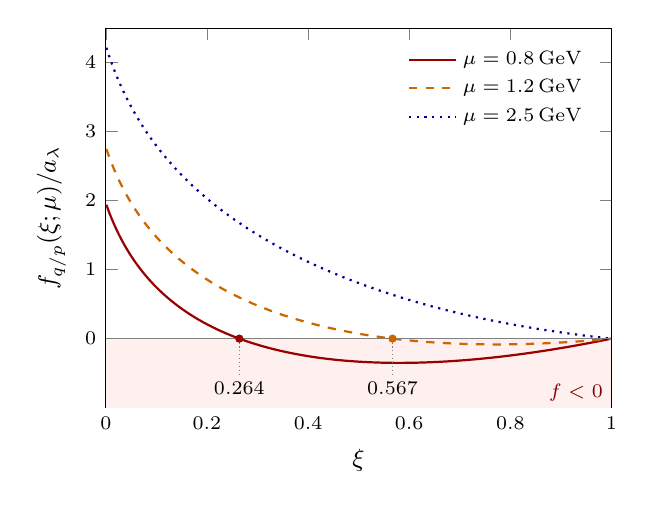
\begin{tikzpicture}
\begin{axis}[width=0.66\textwidth,height=6.4cm,xmin=0,xmax=1,ymin=-1.0,ymax=4.5,
  xlabel={$\xi$},ylabel={$f^{\MSbar}_{q/p}(\xi;\mu)/a_\lambda$},
  xtick={0,0.2,0.4,0.6,0.8,1},ytick={0,1,2,3,4},
  tick label style={font=\scriptsize},label style={font=\small},
  legend style={font=\scriptsize,draw=none,fill=none,at={(0.97,0.97)},anchor=north east},
  legend cell align=left]
\fill[red!6] (axis cs:0,-1.0) rectangle (axis cs:1,0);
\addplot[domain=0.001:0.999,samples=200,thick,red!60!black]{(1-x)*(ln(0.8^2/(2.25*x+0.09*(1-x)-x*(1-x)))-1+(0.3+x)^2/(2.25*x+0.09*(1-x)-x*(1-x)))};
\addlegendentry{$\mu=0.8\,\mathrm{GeV}$}
\addplot[domain=0.001:0.999,samples=200,thick,dashed,orange!80!black]{(1-x)*(ln(1.2^2/(2.25*x+0.09*(1-x)-x*(1-x)))-1+(0.3+x)^2/(2.25*x+0.09*(1-x)-x*(1-x)))};
\addlegendentry{$\mu=1.2\,\mathrm{GeV}$}
\addplot[domain=0.001:0.999,samples=200,thick,dotted,blue!60!black]{(1-x)*(ln(2.5^2/(2.25*x+0.09*(1-x)-x*(1-x)))-1+(0.3+x)^2/(2.25*x+0.09*(1-x)-x*(1-x)))};
\addlegendentry{$\mu=2.5\,\mathrm{GeV}$}
\draw[gray,thin] (axis cs:0,0) -- (axis cs:1,0);
\draw[gray,densely dotted] (axis cs:0.264,0) -- (axis cs:0.264,-0.56);
\draw[gray,densely dotted] (axis cs:0.567,0) -- (axis cs:0.567,-0.56);
\fill[red!60!black] (axis cs:0.264,0) circle[radius=1.5pt];
\fill[orange!80!black] (axis cs:0.567,0) circle[radius=1.5pt];
\node[font=\scriptsize,anchor=north,inner sep=1.5pt] at (axis cs:0.264,-0.56) {$0.264$};
\node[font=\scriptsize,anchor=north,inner sep=1.5pt] at (axis cs:0.567,-0.56) {$0.567$};
\node[font=\scriptsize,text=red!50!black,anchor=south east,inner sep=2pt] at (axis cs:0.995,-1.0) {$f<0$};
\end{axis}
\end{tikzpicture}
\caption{Yukawa 模型中单圈 $\MSbar$ “夸克在核子中”的分布（$m_q=0.3\,\mathrm{GeV}$、$m_p=1.0\,\mathrm{GeV}$、$m_s=1.5\,\mathrm{GeV}$，纵轴以 $a_\lambda=\lambda^2/(16\pi^2)$ 为单位）\cite{CollinsRogersSato2022}：$\mu=0.8\,\mathrm{GeV}$ 时 $\xi>0.264$ 处为负，$\mu=1.2\,\mathrm{GeV}$ 时 $\xi>0.567$ 处为负，$\mu=2.5\,\mathrm{GeV}$ 时处处为正（曲线由 VF-FRO-10 的单圈公式计算）。
“$\MSbar$ 分布在所有标度上非负”因而不成立；足够大标度上的正定性只有部分论证（\cref{prop:front-positivity-large-scale}），一般陈述仍是猜想（\cref{conj:pdf-positivity}）。}
\label{fig:front-yukawa-pdf}
\end{figure}
%%% END fig:front-yukawa-pdf

%%% BEGIN fig:front-dps-double-counting
\begin{figure}[htbp]
\centering
\begin{tikzpicture}[fd,
  fe hadron/.style={draw=black!70,line width=1.5pt,line cap=butt},
  fe dim/.style={draw=gray!55!black,line width=0.5pt,{Stealth[length=3.2pt,width=2.8pt]}-{Stealth[length=3.2pt,width=2.8pt]}},
  fe lab/.style={font=\footnotesize}]
  % ======================= (a) the 1v1 graph =======================
  \begin{scope}
    \node[jet blob,ellipse,minimum width=2.6cm,minimum height=0.8cm,inner sep=0pt] (A) at (0,-2.55) {$A$};
    \node[jetB blob,ellipse,minimum width=2.6cm,minimum height=0.8cm,inner sep=0pt] (B) at (0,2.55) {$B$};
    \node[hard blob,circle,minimum size=0.72cm,inner sep=0pt] (H1) at (-1.45,0) {$H_1$};
    \node[hard blob,circle,minimum size=0.72cm,inner sep=0pt] (H2) at (1.45,0) {$H_2$};
    \coordinate (sA) at (0,-1.3); \coordinate (sB) at (0,1.3);
    \draw[fe hadron] (-2.6,-2.55) -- (A.west);  \draw[fe hadron] (A.east) -- (2.6,-2.55);
    \draw[fe hadron] (-2.6,2.55) -- (B.west);   \draw[fe hadron] (B.east) -- (2.6,2.55);
    \draw[gluon] (A.north) -- (sA);
    \draw[gluon] (B.south) -- (sB);
    % closed quark loop sA -> H1 -> sB -> H2 -> sA
    \draw[quark] (sA) -- (H1.300);
    \draw[quark] (H1.60) -- (sB);
    \draw[quark] (sB) -- (H2.120);
    \draw[quark] (H2.240) -- (sA);
    \node[vertex] at (sA) {}; \node[vertex] at (sB) {};
    \draw[photon] (H1.west) -- (-2.75,0);
    \draw[photon] (H2.east) -- (2.75,0);
    \draw[fe dim] (H1.east) -- node[fe lab,above=1pt] {$y$} (H2.west);
    \node[fe lab,anchor=north west,inner sep=1pt] at (-2.75,-0.05) {$\gamma^*_1$};
    \node[fe lab,anchor=north east,inner sep=1pt] at (2.75,-0.05) {$\gamma^*_2$};
    \node[fe lab,anchor=west,align=left] at (0.2,-1.55) {$1\to2$ 劈裂};
    \node[fe lab,anchor=west,align=left] at (0.2,1.55) {$1\to2$ 劈裂};
    \node[fe lab,align=center,anchor=north] at (0,-3.05) {小 $y$：$F\propto1/y^2$；$y\sim1/Q$ 时此图\\也是单部分子散射的单圈图};
    \node at (0,-4.55) {(a)\ “1v1”图：重复计数};
  \end{scope}
  % ======================= (b) cut-off function and subtraction =======================
  \begin{scope}[xshift=4.5cm,yshift=-2.55cm]
    \fill[red!6] (0.05,0.05) rectangle (1.85,2.45);
    \fill[blue!5] (3.55,0.05) rectangle (6.85,2.45);
    \draw[lcaxis] (0,0) -- (7.2,0) node[right=1pt,fe lab] {$y$};
    \draw[lcaxis] (0,0) -- (0,3.7);
    \draw[gray!60,densely dotted,line width=0.5pt] (0,2.6) -- (6.9,2.6);
    \node[fe lab,anchor=east] at (0,2.6) {$1$};
    \draw[blue!60!black,line width=1.1pt] plot[domain=0.2:6.9,samples=80,smooth] (\x,{2.6/(1+exp(-2.3*(\x-2.6)))});
    \node[fe lab,text=blue!55!black,anchor=south east] at (6.8,2.62) {$\Phi^2(y\nu)$};
    \draw[gray!60!black,line width=0.5pt] (2.6,0.1) -- (2.6,-0.1);
    \node[fe lab,anchor=north] at (2.6,-0.08) {$y\sim1/\nu$，$\nu\sim Q$};
    \node[fe lab,align=center] at (0.95,1.75) {小 $y$};
    \node[fe lab,align=center,text=red!50!black] at (0.95,1.0) {$\sigma_{\rm DPS}\simeq\sigma_{\rm sub}$\\剩 SPS};
    \node[fe lab,align=center] at (5.2,1.75) {大 $y$};
    \node[fe lab,align=center,text=blue!50!black] at (5.2,1.0) {$\sigma_{\rm SPS}\simeq\sigma_{\rm sub}$\\剩 DPS};
    \node[anchor=south] at (3.5,3.75) {$\sigma=\sigma_{\rm SPS}+\sigma_{\rm DPS}-\sigma_{\rm sub}$};
    \node[fe lab,align=center,anchor=north] at (3.5,-0.6) {$\sigma_{\rm sub}$：两个 DPD 都换成固定阶劈裂形式的 DPS 公式};
    \node at (3.5,-2.0) {(b)\ 截断函数 $\Phi(y\nu)$ 与减除项};
  \end{scope}
\end{tikzpicture}
\caption{双部分子散射与单部分子散射在小 $y$ 处的重复计数及其减除：$\sigma=\sigma_{\rm SPS}+\sigma_{\rm DPS}-\sigma_{\rm sub}$（VF-FRO-13）。
(a)~两个强子各经微扰 $1\to2$ 劈裂提供两个部分子（小横向间距 $y$ 处双部分子分布 $F\propto1/y^2$），图中闭合的夸克圈在 $y\sim1/Q$ 时正是单部分子散射的单圈图，两种计算重复计入同一区域；
(b)~DPS 公式中的截断函数 $\Phi(y\nu)$（$\Phi(u)\to1$，$u\gg1$；小 $u$ 处 $\Phi=O(u^\delta)$；曲线为示意）压低小 $y$ 区：小 $y$ 处 $\Phi$ 依赖在 $\sigma_{\rm DPS}$ 与 $\sigma_{\rm sub}$ 之间相消，只剩 SPS，大 $y$ 处 $\sigma_{\rm SPS}\simeq\sigma_{\rm sub}$，只剩 DPS。}
\label{fig:front-dps-double-counting}
\end{figure}
%%% END fig:front-dps-double-counting

%%% BEGIN fig:appM-dependency
\begin{figure}[htbp]
\centering
% Data: the \uses lists of FINAL_OUTLINE_v2 (Ch7 statements, App M, ASSUMPTIONS.md entries):
%  disp  prop:dis-dispersion-np [R,R_cond]  <- W                       (asm only in the node set)
%  eseg  lem:dis-euclid-segment [R,R_def]   <- (def:dis-compton only)
%  oseg  lem:dis-ope-segment [R,R_cond]     <- eseg, O
%  fixn  thm:dis-fixed-n [R,R_cond]         <- oseg, disp, O, W
%  lowm  prop:dis-low-moments [R,R_def]     <- (def:dis-compton only)
%  mnp   thm:dis-moments-np [R,R_cond]      <- fixn, disp, lowm, W, C, O, F, G
%  weak  cor:dis-weak-xspace [R,R_cond]     <- mnp, W, C, O, F
%  oeuc  prop:dis-ope-euclid [A] (by D3)    <- asm:appM-remainder (plain premise, not R_cond and not
%                                              the bottleneck: drawn as an ordinary uses edge)
%  ogi   prop:dis-ope-gi [A]                <- oeuc, asm:appM-brst-ope (bottleneck)
%  ofw   prop:dis-ope-forward [A]           <- oeuc, ogi, asm:appM-forward (bottleneck)
%  mom   thm:dis-moments [R,R_OPE]          <- ofw, thm:dis-ope(=oeuc,ogi,ofw), fixn, disp, mnp, W, C, O, F, G
%  asm:  C <- W;  O <- W, C;  F <- O;  G <- W.
%  W,C,O,F,G = asm:intro-wightman, -composite, -np-ope, -af-coeff, -growth (global, [C]).
\begin{tikzpicture}[
  fe node/.style={rounded corners=1pt,line width=0.6pt,font=\scriptsize,inner xsep=3pt,inner ysep=2.2pt,minimum height=0.5cm,align=center},
  fe asm/.style={fe node,draw=orange!65!black,dash pattern=on 2.5pt off 1.5pt,fill=orange!8},
  fe R/.style={fe node,draw=OliveGreen!75!black,fill=OliveGreen!15},
  fe Rc/.style={fe R,dash pattern=on 2.5pt off 1.5pt},
  fe A/.style={fe node,draw=RoyalBlue!75!black,fill=RoyalBlue!15},
  fe use/.style={draw=gray!55!black,line width=0.6pt,-{Stealth[length=4.2pt,width=3.4pt]},shorten >=0.5pt},
  fe bottle/.style={draw=red!60!black,line width=1.5pt,-{Stealth[length=5.5pt,width=4.6pt]}}]
  \newcommand{\fegl}[1]{\\[-0.5pt]{\color{orange!70!black}\tiny\sffamily\bfseries #1}}
  \newcommand{\fest}{\vphantom{Ag}}% uniform height of the first text line
  % ---------------- assumptions (top row) ----------------
  \node[fe asm] (G) at (0.8,0)  {\fest growth\fegl{G}};
  \node[fe asm] (W) at (2.7,0)  {\fest wightman\fegl{W}};
  \node[fe asm] (C) at (4.6,0)  {\fest composite\fegl{C}};
  \node[fe asm] (O) at (6.5,0)  {\fest np-ope\fegl{O}};
  \node[fe asm] (F) at (8.4,0)  {\fest af-coeff\fegl{F}};
  \node[fe asm] (Rm) at (10.5,0) {\fest remainder};
  \node[fe asm] (Bo) at (12.5,0) {\fest brst-ope};
  \node[fe asm] (Fw) at (14.5,0) {\fest forward};
  \node[font=\footnotesize,anchor=south] at (4.6,0.95) {全局非微扰假设（\texttt{asm:intro-}$\ast$，[C]）};
  \node[font=\footnotesize,anchor=south] at (12.5,0.95) {App M 技术假设（\texttt{asm:appM-}$\ast$，[A]）};
  \draw[fe use] (W) -- (G);
  \draw[fe use] (W) -- (C);
  \draw[fe use] (C) -- (O);
  \draw[fe use] (O) -- (F);
  \draw[fe use] (W.north) .. controls (3.4,0.85) and (5.8,0.85) .. (O.north);
  % ---------------- hadronic (non-perturbative) route ----------------
  \node[fe R]  (eseg) at (1.2,-1.9) {euclid-segment};
  \node[fe Rc] (oseg) at (1.2,-3.4) {ope-segment\fegl{O}};
  \node[fe R]  (lowm) at (1.2,-4.9) {low-moments};
  \node[fe Rc] (disp) at (6.4,-1.9) {dispersion-np\fegl{W}};
  \node[fe Rc] (fixn) at (3.8,-3.4) {fixed-n\fegl{W\,O}};
  \node[fe Rc] (mnp)  at (3.8,-4.9) {moments-np\fegl{W\,C\,O\,F\,G}};
  \node[fe Rc] (weak) at (1.8,-6.4) {weak-xspace\fegl{W\,C\,O\,F}};
  \node[fe R]  (mom)  at (6.4,-6.4) {moments\fegl{W\,C\,O\,F\,G}};
  % ---------------- perturbative route: the three sub-statements of thm:dis-ope ----------------
  \node[fe A] (oeuc) at (10.5,-2.6) {ope-euclid};
  \node[fe A] (ogi)  at (12.5,-2.6) {ope-gi};
  \node[fe A] (ofw)  at (14.5,-2.6) {ope-forward};
  \begin{scope}[on background layer]
    \draw[RoyalBlue!60!black,line width=0.6pt,rounded corners=3pt,fill=RoyalBlue!4] (9.55,-2.05) rectangle (15.4,-3.85);
  \end{scope}
  \node[font=\scriptsize,text=RoyalBlue!50!black,anchor=south east,inner sep=2pt] (gl) at (15.4,-3.85) {thm:dis-ope};
  % edges
  \draw[fe use] (eseg) -- (oseg);
  \draw[fe use] (oseg) -- (fixn);
  \draw[fe use] (disp) -- (fixn);
  \draw[fe use] (disp) -- (mnp);
  \draw[fe use] (fixn) -- (mnp);
  \draw[fe use] (lowm) -- (mnp);
  \draw[fe use] (mnp) -- (weak);
  \draw[fe use] (mnp) -- (mom);
  \draw[fe use] (fixn) -- (mom);
  \draw[fe use] (disp) -- (mom);
  \draw[fe use] (oeuc) -- (ogi);
  \draw[fe use] (ogi) -- (ofw);
  \draw[fe use] (oeuc.south) .. controls (11.2,-3.65) and (13.8,-3.65) .. (ofw.south);
  \draw[fe use] (9.55,-3.6) -- (mom);
  \draw[fe use] (Rm) -- (oeuc);
  \draw[fe bottle] (Bo) -- (ogi);
  \draw[fe bottle] (Fw) -- (ofw);
  % ---------------- legend ----------------
  \begin{scope}[shift={(9.7,-4.75)}]
    \node[fe R,minimum width=0.55cm,minimum height=0.32cm,inner sep=0pt] at (0,0) {};
    \node[font=\scriptsize,anchor=west] at (0.32,0) {R 严格};
    \node[fe A,minimum width=0.55cm,minimum height=0.32cm,inner sep=0pt] at (1.8,0) {};
    \node[font=\scriptsize,anchor=west] at (2.12,0) {A 全阶论证};
    \node[fe Rc,minimum width=0.55cm,minimum height=0.32cm,inner sep=0pt] at (4.1,0) {};
    \node[font=\scriptsize,anchor=west] at (4.42,0) {$R_{\mathrm{cond}}$};
    \node[fe asm,minimum width=0.55cm,minimum height=0.32cm,inner sep=0pt] at (0,-0.5) {};
    \node[font=\scriptsize,anchor=west] at (0.32,-0.5) {编号假设};
    \node[font=\scriptsize,anchor=west] at (1.75,-0.5) {{\color{orange!70!black}\sffamily\bfseries W\,C\,O\,F\,G}：所用全局假设};
    \draw[fe use] (-0.3,-1.0) -- (0.3,-1.0);
    \node[font=\scriptsize,anchor=west] at (0.32,-1.0) {依赖};
    \draw[fe bottle] (1.25,-1.0) -- (1.85,-1.0);
    \node[font=\scriptsize,anchor=west] at (1.87,-1.0) {瓶颈：[A] 地位即该假设的地位};
  \end{scope}
\end{tikzpicture}
\caption{DIS 矩定理对编号假设的依赖（据各陈述所列的“依赖”绘制；节点只写标签去掉前缀 \texttt{prop:dis-}、\texttt{asm:intro-} 等后的部分）：\cref{thm:dis-moments} 的微扰部分只依赖 OPE 的三个子陈述（蓝框，即 \cref{thm:dis-ope}），它们在编号假设中只用到 App M 的三个技术假设，其中 \cref{asm:appM-brst-ope}、\cref{asm:appM-forward} 是相应 [A] 陈述的瓶颈（粗红线）；非微扰的固定 $n$ 定理（\cref{thm:dis-fixed-n}）依赖 Wightman 公理（W）与非微扰 OPE（O），$n<n_0$ 的矩（\cref{thm:dis-moments-np}）还依赖增长条件（G）。
框色为严格性标签，虚线框为 $R_{\mathrm{cond}}$ 条件定理，橙色虚线框为编号假设；节点第二行的橙色字母标出该陈述直接使用的全局假设（W、C、O、F、G 对应上排五个全局假设），其余依赖画为由前提指向陈述的箭头。}
\label{fig:appM-dependency}
\end{figure}
%%% END fig:appM-dependency

%%% BEGIN fig:appM-forest
\begin{figure}[htbp]
\centering
\begin{tikzpicture}[fd,
  fe reg/.style={region,line width=0.7pt},
  fe aux/.style={draw=gray!55!black,line width=0.7pt,dash pattern=on 1pt off 1.6pt},
  fe lab/.style={font=\footnotesize}]
  % ======================= (a) a forest of a two-loop graph =======================
  % forward Compton graph (uncut): q enters at V_A, leaves at V_B; vertex correction gamma_1 at V_A,
  % gamma_2 = gamma_1 + the struck-quark line b->V_B (contains both current vertices; not 1PI by
  % itself, but gamma_2 + l_x is 1PI: an AB part, omega = D - sum_E d_e = 2 - 3 = -1, subtracted
  % only in N_a with delta_a = a - 3), self-energy gamma_3 on the incoming quark line (no common
  % vertex with gamma_2; omega(gamma_1) = 0, omega(gamma_3) = 1).
  \begin{scope}
    \coordinate (VA) at (-1.25,2.3); \coordinate (VB) at (1.25,2.3);
    \coordinate (a) at (-1.25,1.35); \coordinate (b) at (-0.05,2.3);
    \coordinate (c) at (-1.25,-0.5); \coordinate (d) at (-1.25,0.4);
    \coordinate (Ein) at (-1.25,-1.4); \coordinate (Eout) at (1.25,-1.4);
    % subgraph boxes (drawn first)
    \draw[fe reg,blue!55!black] (-1.55,1.05) rectangle (0.3,2.6);
    \draw[fe reg] (-1.85,0.8) rectangle (1.6,2.9);
    \draw[fe reg,orange!75!black] (-2.05,-0.78) rectangle (-0.93,0.67);
    % lines
    \draw[photon] (-2.45,3.45) -- (VA);
    \draw[photon] (VB) -- (2.45,3.45);
    \draw[quark=0.5] (Ein) -- (c);
    \draw[quark] (c) -- (d);
    \draw[quark=0.55] (d) -- (a);
    \draw[quark=0.6] (a) -- (VA);
    \draw[quark=0.6] (VA) -- (b);
    \draw[quark] (b) -- (VB);
    \draw[quark=0.62] (VB) -- (Eout);
    \draw[gluon] (a) .. controls (-0.6,1.37) and (-0.1,1.75) .. (b);
    \draw[gluon] (c) .. controls (-1.98,-0.4) and (-1.98,0.3) .. (d);
    \foreach \p in {VA,VB,a,b,c,d} \node[vertex] at (\p) {};
    \path[mom'={$q$},mom sep=0.24cm] (-2.45,3.45) -- (VA);
    \path[mom'={$q$},mom sep=0.24cm] (VB) -- (2.45,3.45);
    \path[mom'={$p$},mom pos=0.42] (Ein) -- (c);
    \path[mom={$p$},mom pos=0.72] (VB) -- (Eout);
    \node[fe lab,anchor=north west,inner sep=1pt] at (-1.2,2.24) {$V_A$};
    \node[fe lab,anchor=north east,inner sep=1pt] at (1.2,2.24) {$V_B$};
    \node[fe lab,text=blue!50!black,anchor=south east,inner sep=1.5pt] at (0.3,1.05) {$\gamma_1$};
    \node[fe lab,anchor=west,inner sep=2pt] at (1.6,1.15) {$\gamma_2$};
    \node[fe lab,text=orange!65!black,anchor=east,inner sep=2pt] at (-2.05,-0.05) {$\gamma_3$};
    \node[fe lab,anchor=north] at (0.05,-1.75) {森林 $F=\{\gamma_1,\gamma_2,\gamma_3\}$：$\gamma_1\subset\gamma_2$，$\gamma_3\cap\gamma_2=\varnothing$};
    \node[anchor=north] at (0.05,-2.3) {$R_\Gamma=\sum_F\prod^{\curvearrowleft}_{\gamma\in F}\big(-t^{\delta(\gamma)}_\gamma\big)\,I_\Gamma$};
    \node at (0.05,-3.35) {(a)\ 森林：两两嵌套或不相交};
  \end{scope}
  % ======================= (b) frozen-q bilocal normal product =======================
  \begin{scope}[xshift=7.6cm]
    \coordinate (VA) at (-1.0,1.85); \coordinate (VB) at (1.0,1.85);
    \coordinate (u) at (-1.0,0.65); \coordinate (w) at (1.0,0.65);
    \draw[fe reg,line width=0.8pt] (-1.38,0.35) rectangle (1.38,2.2);
    \draw[quark] (-1.95,-0.35) -- (u);
    \draw[quark] (w) -- (1.95,-0.35);
    \draw[quark] (u) -- (VA);
    \draw[quark] (VA) -- (VB);
    \draw[quark] (VB) -- (w);
    \draw[gluon] (u) -- (w);
    \node[vertex] at (u) {}; \node[vertex] at (w) {};
    % auxiliary line l_x carrying the frozen external momentum q
    \draw[fe aux] (VA) .. controls (-0.85,3.25) and (0.85,3.25) .. (VB);
    \path[mom={$q$},mom sep=0.2cm] (VA) .. controls (-0.85,3.25) and (0.85,3.25) .. (VB);
    \node[opvertex] at (VA) {}; \node[opvertex] at (VB) {};
    \node[fe lab,anchor=east,inner sep=2pt] at (-1.38,1.85) {$A(x)$};
    \node[fe lab,anchor=west,inner sep=2pt] at (1.38,1.85) {$B(0)$};
    \node[fe lab,anchor=west,inner sep=1pt,text=gray!40!black] at (0.82,2.85) {$\ell_x$：$\ee^{-\ii q\cdot x}$};
    \path[mom={$p_1$},mom pos=0.45] (-1.95,-0.35) -- (u);
    \path[mom'={$p_2$},mom pos=0.55] (w) -- (1.95,-0.35);
    \node[fe lab,anchor=north,inner sep=2pt] at (0,0.35) {AB 部分 $\gamma$};
    \node[fe lab,align=center,anchor=north] at (0,-0.65) {只对外动量 $p$（不对 $q$）作 Taylor 减除：\\$t^{\delta_a(\gamma)}_p$，$\delta_a(\gamma)=a-\sum_{E(\gamma)}d_e$};
    \node[fe lab,align=center,anchor=north,text=red!60!black] at (0,-1.75) {减除次数须对顶点可加};
    \node at (0,-3.35) {(b)\ 冻结 $q$ 的双局域正规乘积 $N_a[A(x)B(0)]$};
  \end{scope}
\end{tikzpicture}
\caption{BPHZ 森林公式与正规乘积（示意）：(a)~森林是两两嵌套或不相交的子图（重整化部分；在正规乘积中还包括 AB 部分）的集合，例如紫外发散的顶点修正 $\gamma_1$ 与自能 $\gamma_3$，以及包含 $\gamma_1$ 与两个流顶点 $V_A$、$V_B$ 的 AB 部分 $\gamma_2$（$\gamma_3$ 与 $\gamma_2$ 无公共顶点）；$R_\Gamma$ 中较小的子图先作用（$\curvearrowleft$），大动量 $q$ 自 $V_A$ 流入、自 $V_B$ 流出；
(b)~冻结 $q$ 的双局域正规乘积中，含两个流顶点的子图（AB 部分，加上辅助线 $\ell_x$ 后为单粒子不可约）只对外动量 $p$ 作 Taylor 减除，$q$ 不展开。
减除次数必须对顶点可加（$\delta(\gamma)=\omega(\gamma)+\sum_{v\in V(\gamma)}c_v$），否则可构造反例（\cref{ex:appM-nonadditive}）。}
\label{fig:appM-forest}
\end{figure}
%%% END fig:appM-forest

%%% BEGIN fig:appM-handbag-ab
\begin{figure}[htbp]
\centering
\begin{tikzpicture}[fd,
  fe hadron/.style={draw,solid,line width=1.5pt,line cap=butt},
  fe reg/.style={region,line width=0.8pt},
  fe map/.style={draw=gray!60!black,line width=0.7pt,-{Stealth[length=5pt,width=4pt]}},
  fe lab/.style={font=\footnotesize}]
  % ======================= (a) handbag as an AB part =======================
  \begin{scope}
    \coordinate (VA) at (-1.15,2.05); \coordinate (VB) at (1.15,2.05);
    \coordinate (BL) at (-0.62,0.36); \coordinate (BR) at (0.62,0.36);
    \draw[fe hadron] (-2.3,0) -- (-0.8,0);
    \draw[fe hadron] (0.8,0) -- (2.3,0);
    \draw[quark=0.55] (BL) -- (VA);
    \draw[quark=0.55] (VA) -- (VB);
    \draw[quark=0.55] (VB) -- (BR);
    \draw[photon] (-2.25,3.15) -- (VA);
    \draw[photon] (VB) -- (2.25,3.15);
    \draw[hadron blob] (0,0) ellipse[x radius=0.95,y radius=0.45];
    \node[vertex] at (VA) {}; \node[vertex] at (VB) {};
    \draw[fe reg,red!60!black] (-1.5,1.72) rectangle (1.5,2.72);
    \path[mom'={$q$},mom sep=0.22cm] (-2.25,3.15) -- (VA);
    \path[mom={$q$},mom sep=0.22cm] (VB) -- (2.25,3.15);
    \path[mom={$k$},mom pos=0.45] (BL) -- (VA);
    \path[mom={$k$},mom pos=0.55] (VB) -- (BR);
    \path[mom={$k+q$},mom pos=0.5,mom sep=0.2cm] (VA) -- (VB);
    \path[mom={$P$},mom sep=0.28cm] (-2.3,0) -- (-1.15,0);
    \path[mom={$P$},mom sep=0.28cm] (1.15,0) -- (2.3,0);
    \node[fe lab,text=red!55!black,anchor=north,align=center] at (0,1.66) {AB 部分 $\gamma$\\（$q$ 冻结）};
    \node[fe lab,text=red!55!black,anchor=west,inner sep=2pt] at (1.5,2.05) {$\to C^{(n)}(q)$};
    \node[fe lab,anchor=north,align=center] at (0,-0.55) {其余部分 $\to\langle P|O^{(n)}|P\rangle$};
    % contraction of gamma: local operator vertex
    \draw[fe map] (2.45,1.2) -- node[above,fe lab,inner sep=2pt] {收缩 $\gamma$} (3.6,1.2);
    \begin{scope}[shift={(4.65,0)}]
      \coordinate (O) at (0,1.7);
      \draw[quark=0.55] (-0.45,0.33) -- (O);
      \draw[quark=0.55] (O) -- (0.45,0.33);
      \draw[fe hadron] (-1.0,0) -- (-0.55,0);
      \draw[fe hadron] (0.55,0) -- (1.0,0);
      \draw[hadron blob] (0,0) ellipse[x radius=0.65,y radius=0.36];
      \node[opvertex,minimum size=8pt] at (O) {};
      \node[fe lab,anchor=south,inner sep=3pt] at (O) {$O^{(n)}$};
      \node[fe lab,anchor=north,align=center] at (0,-0.55) {$\propto A^{(n)}$};
    \end{scope}
    \node at (1.4,-1.5) {(a)\ AB 部分（正规乘积的语言）};
  \end{scope}
  % ======================= (b) handbag as a reduced graph =======================
  \begin{scope}[xshift=10.1cm]
    \coordinate (H) at (0,2.05);
    \draw[fe hadron] (-2.3,0) -- (-1.0,0);
    \draw[fe hadron] (1.0,0) -- (2.3,0);
    \draw[quark=0.5] (-0.42,0.38) -- ($(H)+(-0.3,-0.3)$);
    \draw[quark=0.5] ($(H)+(0.3,-0.3)$) -- (0.42,0.38);
    \draw[photon] (-2.05,3.05) -- ($(H)+(-0.38,0.18)$);
    \draw[photon] ($(H)+(0.38,0.18)$) -- (2.05,3.05);
    \draw[jet blob] (0,0) ellipse[x radius=1.1,y radius=0.45];
    \draw[hard blob] (H) circle[radius=0.42];
    \node at (H) {$H$};
    \node at (0,0) {$J_A$};
    \path[mom'={$q$},mom sep=0.22cm] (-2.05,3.05) -- ($(H)+(-0.38,0.18)$);
    \path[mom={$q$},mom sep=0.22cm] ($(H)+(0.38,0.18)$) -- (2.05,3.05);
    \path[mom={$P$},mom sep=0.28cm] (-2.3,0) -- (-1.3,0);
    \path[mom={$P$},mom sep=0.28cm] (1.3,0) -- (2.3,0);
    \node[fe lab,anchor=west,inner sep=2pt] at (0.45,2.05) {硬顶点 $\to C^{(n)}$};
    \node[fe lab,anchor=west,align=left,text=blue!50!black] at (0.55,1.0) {共线线\\（平行于 $n_A$）};
    \node[fe lab,anchor=north,align=center] at (0,-0.55) {靶的共线子图 $\to A^{(n)}$};
    \node at (0,-1.5) {(b)\ 约化图（区域的语言）};
  \end{scope}
\end{tikzpicture}
\caption{手提包图（前向 Compton 振幅，未切割）的两种读法：(a)~作为正规乘积展开中的 AB 部分——含两个流顶点的子图 $\gamma$（$q$ 冻结在其中）给出系数 $C^{(n)}(q)$，把 $\gamma$ 收缩为一点后其余部分给出局域算符 $O^{(n)}$ 的矩阵元（$\propto A^{(n)}$）；
(b)~作为区域分析中的约化图——硬顶点 $H$ 与靶（沿 $+z$ 运动）的共线子图 $J_A$ 由平行于 $n_A$ 的共线线相连。
在有质量模型中两种读法的重叠由超减除分开；无质量 QCD 中还需要红外抵消项（\cref{sec:appM-massless}）。}
\label{fig:appM-handbag-ab}
\end{figure}
%%% END fig:appM-handbag-ab

%%% BEGIN fig:appM-euclid-forward
\begin{figure}[htbp]
\centering
\begin{tikzpicture}[fd,
  fe big/.style={draw=blue!60!black,line width=1.1pt,-{Stealth[length=6.5pt,width=5pt]}},
  fe ghostq/.style={draw=blue!45,line width=0.6pt,dash pattern=on 2pt off 1.5pt,-{Stealth[length=4.5pt,width=3.6pt]}},
  fe small/.style={draw,line width=0.9pt,-{Stealth[length=5pt,width=4pt]}},
  fe exc/.style={draw=red!60!black,line width=0.6pt,dash pattern=on 3pt off 2pt},
  fe lab/.style={font=\footnotesize}]
  % ======================= (a) Euclidean, non-exceptional =======================
  \begin{scope}
    % 2D projection of Euclidean momentum space
    \draw[blue!55!black,line width=0.6pt,dash pattern=on 3pt off 2pt] (6:3.45) arc[start angle=6,end angle=54,radius=3.45];
    \draw[fe ghostq] (0,0) -- (14:3.4);
    \draw[fe ghostq] (0,0) -- (46:3.4);
    \draw[fe big] (0,0) -- (30:3.4);
    \node[anchor=south west,inner sep=1pt,text=blue!55!black] at (30:3.42) {$q=|q|\,\hat q$};
    \node[fe lab,text=blue!50!black,anchor=north west,inner sep=2pt] at (6:3.45) {$\hat q$ 任意};
    \draw[fe small] (0,0) -- (118:0.95) node[anchor=south east,inner sep=1pt] {$p_1$};
    \draw[fe small] (0,0) -- (205:0.9) node[anchor=north east,inner sep=1pt] {$p_2$};
    \node[circle,fill=black,inner sep=0pt,minimum size=3pt] at (0,0) {};
    \node[fe lab,anchor=north east,inner sep=2pt] at (0.05,-0.08) {$0$};
    \node[fe lab,align=center,anchor=north] at (1.35,-0.95) {余项 $O(|q|^{D-1-a}\ln^k|q|)$，对 $\hat q$ 一致};
    % inset: configuration space of the external momenta (exceptional set = linear subspaces)
    \begin{scope}[shift={(-0.7,2.35)}]
      \fill[gray!7] (-1.3,-0.8) rectangle (1.3,0.8);
      \begin{scope}
        \clip (-1.3,-0.8) rectangle (1.3,0.8);
        \foreach \t in {15,72,140} \draw[fe exc] (\t:-1.6) -- (\t:1.6);
      \end{scope}
      \fill[green!18,draw=green!45!black,line width=0.5pt] (43:0.78) ellipse[x radius=0.24,y radius=0.15];
      \node[circle,fill=black,inner sep=0pt,minimum size=2.6pt] at (43:0.78) {};
      \node[font=\scriptsize,anchor=west,inner sep=1.5pt] at ($(43:0.78)+(0.24,0)$) {$K$};
      \node[circle,fill=red!60!black,inner sep=0pt,minimum size=2.4pt] at (0,0) {};
      \node[font=\scriptsize,text=red!55!black,anchor=south west,inner sep=1pt] at (-1.3,-0.8) {例外集};
      \node[font=\scriptsize,anchor=south,inner sep=2pt,align=center] at (0,0.8) {外动量构型空间（示意）};
    \end{scope}
    \node at (1.35,-2.0) {(a)\ 欧氏、非例外外动量};
  \end{scope}
  % ======================= (b) forward on-shell partonic kinematics =======================
  \begin{scope}[xshift=8.4cm]
    \coordinate (VA) at (-1.0,2.1); \coordinate (VB) at (1.0,2.1);
    \coordinate (Pin) at (-1.75,0.0); \coordinate (Pout) at (1.75,0.0);
    \draw[red!60!black,line width=0.8pt,dash pattern=on 3pt off 2pt,rounded corners=4pt] (-2.15,-0.25) rectangle (2.15,0.75);
    \draw[photon] (-2.15,3.2) -- (VA);
    \draw[photon] (VB) -- (2.15,3.2);
    \draw[quark=0.62] (Pin) -- (VA);
    \draw[quark=0.55] (VA) -- (VB);
    \draw[quark=0.45] (VB) -- (Pout);
    \node[vertex] at (VA) {}; \node[vertex] at (VB) {};
    \path[mom'={$q$},mom sep=0.22cm] (-2.15,3.2) -- (VA);
    \path[mom={$q$},mom sep=0.22cm] (VB) -- (2.15,3.2);
    \path[mom={$p+q$},mom sep=0.2cm] (VA) -- (VB);
    \path[mom={$p$},mom pos=0.6] (Pin) -- (VA);
    \path[mom={$p$},mom pos=0.4] (VB) -- (Pout);
    \node[fe lab,anchor=north,inner sep=2pt] at (0,0.62) {$p^2=0$};
    \node[fe lab,text=red!55!black,anchor=north,align=center] at (0,-0.3) {两条外部部分子线：$p+(-p)=0$，例外动量};
    \node[fe lab,anchor=north,align=center] at (0,-0.95) {余项估计：需\cref{asm:appM-forward}};
    \node at (0,-2.0) {(b)\ 前向在壳部分子矩阵元};
  \end{scope}
\end{tikzpicture}
\caption{欧氏非例外动量与前向在壳运动学：(a)~微扰 OPE 的定理形式（\cref{prop:dis-ope-euclid}）适用于欧氏、非例外的外动量——外动量取在避开例外集（某个真部分和为零；在构型空间中是过原点的线性子空间，图中虚线）的紧集 $K$ 内，$|q|\to\infty$ 时余项在方向 $\hat q$ 上一致；
(b)~DIS 所需的前向在壳部分子矩阵元（入射与出射动量同为 $p$，$p^2=0$）是例外构型，欧氏定理不直接适用，其余项估计是编号假设（\cref{asm:appM-forward}；$O(\alpha_s)$ 已精确到 $\varepsilon$ 地检验至 $N\le8$，VF-DIS-13）。}
\label{fig:appM-euclid-forward}
\end{figure}
%%% END fig:appM-euclid-forward

%%% BEGIN fig:appN-triangle-regions
\begin{figure}[htbp]
\centering
% Schematic (k_T=0 section): N_C1={|k^-|+|k_T|<=lam^(1/3)}, N_C2={|k^+|+|k_T|<=lam^(1/3)},
% N_S={||k||<=lam^(1/9)} (def:method-neighbourhoods, beta_S=1/9, beta_C=1/3; units of Q);
% drawn half-width 0.36 cm, radius 1.1 cm. Pinch sets: pi_C1 = {0<k^+<P}, pi_C2 = {0<k^-<P'}.
\begin{tikzpicture}[fd,
  fe tube A/.style={fill=blue!12,draw=blue!45!black,line width=0.4pt},
  fe tube B/.style={fill=orange!18,draw=orange!70!black,line width=0.4pt},
  fe ball/.style={fill=green!15,draw=green!45!black,line width=0.5pt},
  fe pinch/.style={line width=2.2pt,line cap=round},
  fe dim/.style={draw,line width=0.45pt,{Stealth[length=3pt,width=2.6pt]}-{Stealth[length=3pt,width=2.6pt]}},
  fe box/.style={draw,rounded corners=2pt,line width=0.5pt,align=left,font=\footnotesize,inner sep=3pt,text width=5.15cm},
  fe lead/.style={draw=gray!60!black,line width=0.45pt},
  fe lab/.style={font=\footnotesize}]
  \def\fehw{0.36}\def\feR{1.1}
  % neighbourhoods (strips along the full axes in the window, ball on top)
  \fill[fe tube A] (-1.4,-\fehw) rectangle (6.0,\fehw);
  \fill[fe tube B] (-\fehw,-1.4) rectangle (\fehw,4.5);
  \draw[blue!45!black,line width=0.4pt] (-1.4,\fehw) -- (6.0,\fehw) (-1.4,-\fehw) -- (6.0,-\fehw);
  \draw[orange!70!black,line width=0.4pt] (-\fehw,-1.4) -- (-\fehw,4.5) (\fehw,-1.4) -- (\fehw,4.5);
  \draw[fe ball] (0,0) circle[radius=\feR];
  % axes
  \draw[lcaxis] (-1.4,0) -- (6.35,0) node[right=1pt] {$k^+$};
  \draw[lcaxis] (0,-1.4) -- (0,4.8) node[above=1pt] {$k^-$};
  % pinch sets
  \draw[fe pinch,blue!60!black] (0,0) -- (4.6,0);
  \draw[fe pinch,orange!80!black] (0,0) -- (0,3.4);
  \fill (0,0) circle[radius=2.2pt];
  \draw[line width=0.5pt] (4.6,0.12) -- (4.6,-0.12); \draw[line width=0.5pt] (0.12,3.4) -- (-0.12,3.4);
  \node[fe lab,anchor=south,inner sep=2pt] at (4.6,\fehw) {$P$};
  \node[fe lab,anchor=east,inner sep=2pt] at (-\fehw,3.4) {$P'$};
  \node[fe lab,text=blue!55!black,anchor=south,inner sep=2pt] at (3.8,\fehw) {$\pi_{C_1}$};
  \node[fe lab,text=orange!65!black,anchor=west,inner sep=2pt] at (\fehw,3.05) {$\pi_{C_2}$};
  \node[fe lab,anchor=north east,inner sep=1.5pt] at (-0.03,-0.03) {$\pi_S$};
  % dimensions
  \draw[fe dim] (2.4,0) -- (2.4,\fehw);
  \node[font=\scriptsize,anchor=south west,inner sep=1pt] at (2.42,\fehw) {$\lambda^{1/3}$};
  \draw[fe dim] (0,0) -- (135:\feR);
  \node[font=\scriptsize,anchor=south east,inner sep=1pt] at (135:\feR) {$\lambda^{1/9}$};
  % region labels
  \node[fe lab] at (-0.66,-0.68) {$U_S$};
  \node[fe lab,text=blue!50!black,anchor=south,inner sep=2pt] at (1.45,\fehw) {$U_{C_1}$};
  \node[fe lab,text=orange!60!black,anchor=east,inner sep=2pt] at (-\fehw,2.0) {$U_{C_2}$};
  \node[fe lab] at (2.9,3.3) {$U_H$};
  % boxes with the grouped expressions
  \node[fe box,anchor=west] (bH) at (7.35,3.95) {$U_H$：(CS1)\ $(1-T_H)X_H$，\\ \quad$X_H=\Gamma-C_S\Gamma-C_{C_1}\Gamma-C_{C_2}\Gamma$};
  \node[fe box,anchor=west,fill=orange!10] (bB) at (7.35,2.55) {$U_{C_2}$：(CS1)\ $(1-T_{C_2})(\Gamma-C_S\Gamma)$\\ \quad\ \ \,(CS2)\ $C_{C_1}\Gamma,\ C_H\Gamma$};
  \node[fe box,anchor=west,fill=blue!8] (bA) at (7.35,1.15) {$U_{C_1}$：(CS1)\ $(1-T_{C_1})(\Gamma-C_S\Gamma)$\\ \quad\ \ \,(CS2)\ $C_{C_2}\Gamma,\ C_H\Gamma$};
  \node[fe box,anchor=west,fill=green!10] (bS) at (7.35,-0.5) {$U_S$：(CS1)\ $(1-T_S)\Gamma$\\ \quad\ \,(CS2)\ $C_{C_1}\Gamma,\ C_{C_2}\Gamma,\ C_H\Gamma$};
  \draw[fe lead] (bH.west) -- (3.25,3.38);
  \draw[fe lead] (bB.west) -- (0.22,2.35);
  \draw[fe lead] (bA.west) -- (5.3,0.18);
  \draw[fe lead] (bS.west) -- (-45:0.98);% runs below the tube N_C1 to the ball N_S
  \fill[gray!60!black] (3.25,3.38) circle[radius=1pt] (0.22,2.35) circle[radius=1pt] (5.3,0.18) circle[radius=1pt] (-45:0.98) circle[radius=1pt];
  % note on the soft approximation
  \node[fe lab,anchor=north west,align=left] (nt) at (-1.4,-1.75) {原点附近：软近似只在穿过 $\Real k^-\sim\kT^2/(4k^+)$ 的围道上成立，在实轴 $k^-\approx0$ 处不成立};
\end{tikzpicture}
\caption{单圈离壳三角图（$p_1=(P,-\frac{m^2}{2P},\mathbf 0_T)$，$p_2=(\frac{m^2}{2P'},-P',\mathbf 0_T)$）的区域与邻域（$k_T=0$ 截面，示意）：$\pi_{C_1}$、$\pi_{C_2}$ 为两条共线钳夹线，$\pi_S=\{0\}$；$N_{C_1}=\{|k^-|+|\mathbf k_T|\le\lambda^{1/3}\}$、$N_{C_2}=\{|k^+|+|\mathbf k_T|\le\lambda^{1/3}\}$ 为半宽 $\lambda^{1/3}$ 的管（蓝、橙），$N_S$ 为半径 $\lambda^{1/9}$ 的球（绿；以 $Q$ 为单位），支配集 $U_S=N_S$、$U_{C_i}=N_{C_i}\setminus N_S$，$U_H$ 为其余部分。
每个支配集 $U_R$ 上标出提供小因子的分组表达式，即 (CS1)(CS2) 在本例中的具体形式（\cref{def:method-collins-conditions}）。}
\label{fig:appN-triangle-regions}
\end{figure}
%%% END fig:appN-triangle-regions

%%% BEGIN fig:appN-triangle-remainder
\begin{figure}[htbp]
\centering
% Data: inline coordinates from spec_v2/checks/fig_data.py (log: checks/fig_data.log), i.e. the
% closed form Q^2 I = Phi^(1)(t,t) (VF-REF-2) minus the Collins subtraction terms written with
% tilde Q^2 (VF-REF-3); dashed curves are the NLP expansions of prop:appN-triangle-exact (c)(d).
% Recomputed independently with mpmath (dps=40): e.g. t=0.01: -3.8972454 and 27.313006.
\begin{tikzpicture}
\begin{axis}[name=A,width=0.48\textwidth,height=5.6cm,xmode=log,xmin=1e-5,xmax=0.2,ymin=-9,ymax=-3.4,
  xlabel={$t=m^2/Q^2$},ylabel={$Q^2\!\int r\,/\,t$},tick label style={font=\scriptsize},label style={font=\small},
  legend style={font=\scriptsize,draw=none,fill=none,at={(0.03,0.03)},anchor=south west},legend cell align=left]
\addplot[only marks,mark=*,mark size=1.2pt] coordinates {(1.0e-5,-3.99879) (1.77828e-5,-3.99808) (3.16228e-5,-3.99697) (5.62341e-5,-3.99527) (0.0001,-3.99268) (0.000177828,-3.98881) (0.000316228,-3.98313) (0.000562341,-3.97501) (0.001,-3.96377) (0.00177828,-3.94895) (0.00316228,-3.93081) (0.00562341,-3.91148) (0.01,-3.89725) (0.0177828,-3.90336) (0.0316228,-3.96534) (0.0562341,-4.17112) (0.1,-4.7898) (0.15,-6.06052) (0.2,-8.80249)};
\addlegendentry{精确}
\addplot[domain=1e-5:0.2,samples=80,thick,dashed,red!60!black]{-4+x*(ln(1/x)^2-15+pi^2/3)};
\addlegendentry{$-4+t(L^2-15+\frac{\pi^2}3)$}
\end{axis}
\begin{axis}[name=B,at={(A.east)},anchor=west,xshift=1.7cm,width=0.48\textwidth,height=5.6cm,xmode=log,xmin=1e-5,xmax=0.2,ymin=0,ymax=235,
  xlabel={$t=m^2/Q^2$},ylabel={NLP 系数},tick label style={font=\scriptsize},label style={font=\small},
  legend style={font=\scriptsize,draw=none,fill=none,at={(0.97,0.97)},anchor=north east},legend cell align=left]
\addplot[only marks,mark=*,mark size=1.2pt] coordinates {(1.0e-5,221.629) (1.77828e-5,198.089) (3.16228e-5,175.876) (5.62341e-5,154.992) (0.0001,135.438) (0.000177828,117.216) (0.000316228,100.33) (0.000562341,84.7839) (0.001,70.5819) (0.00177828,57.7299) (0.00316228,46.2333) (0.00562341,36.0952) (0.01,27.313) (0.0177828,19.8734) (0.0316228,13.745) (0.0562341,8.87051) (0.1,5.16015) (0.15,3.17897) (0.2,2.05715)};
\addlegendentry{精确 $(Q^2I-L^2-\frac{\pi^2}3)/t$}
\addplot[domain=1e-5:0.2,samples=80,thick,dashed,blue!60!black]{2*ln(1/x)^2-4*ln(1/x)-4+2*pi^2/3};
\addlegendentry{$2L^2-4L-4+\frac{2\pi^2}3$}
\end{axis}
\node[anchor=north] at ([yshift=-1.18cm]A.south) {(a)\ 余项：次领头幂次无对数};
\node[anchor=north] at ([yshift=-1.18cm]B.south) {(b)\ 原积分：次领头系数含 $L^2$、$L$};
\end{tikzpicture}
\caption{单圈离壳三角图的 Collins 减除（$t=m^2/Q^2$，$L=\ln(1/t)$）：(a)~精确余项 $Q^2\!\int r/t$ 趋于 $-4$，修正为 $t(L^2-15+\frac{\pi^2}3)$——余项在次领头幂次没有对数；
(b)~原积分 $Q^2I$ 的次领头系数按 $2L^2-4L-4+\frac{2\pi^2}3$ 增长，这些对数完全由用精确运动学（$\tilde Q^2\neq Q^2$）写出的减除项再现（\cref{prop:appN-triangle-exact}，VF-REF-2，VF-REF-3）。}
\label{fig:appN-triangle-remainder}
\end{figure}
%%% END fig:appN-triangle-remainder

%%% BEGIN fig:appN-chain-pairing
\begin{figure}[htbp]
\centering
% The nine-region poset of fig:method-hasse (same node layout; line-wise order S<C_1,C_2<H,
% C_1^C_2=S; 12 covering edges), R_0=(C_1,C_1).  Checked with non-commuting symbols (sympy):
% comparable with R_0: down R_0={(S,S),(C_1,S)}, up R_0={(H,C_1),(H,H)} (up R={X>R});
% incomparable: (C_2,S),(H,S),(C_2,C_2),(H,C_2) with meets (S,S),(C_1,S),(S,S),(C_1,S);
% every pinch set contains pi_(S,S) ((S,S) is a common lower bound), hence I'={all four}, I''=empty;
% r = O_up(R_0)[(1-T_R0)X_R0] - sum_{R in I'} O_up(R) T_R[(1-T_R^)X_R^] holds identically;
% O_up(R_0)=(1-T_HH)(1-T_HC1), X_R0=(1-T_C1S)(1-T_SS)Gamma, X_(C1,S)=(1-T_SS)Gamma, X_(S,S)=Gamma.
\begin{tikzpicture}[
  fe node/.style={draw=gray!60!black,fill=white,rounded corners=2.5pt,line width=0.6pt,inner sep=2.5pt,
    minimum width=1.35cm,minimum height=0.55cm,font=\small},
  fe R0/.style={fe node,draw=red!60!black,fill=red!8,line width=1.2pt},
  fe Ip/.style={fe node,draw=blue!60!black,fill=blue!10,line width=0.8pt},
  fe edge/.style={draw=gray!55!black,line width=0.7pt},
  fe chain/.style={draw=red!60!black,line width=1.6pt},
  fe lab/.style={font=\footnotesize}]
  % ======================= the poset =======================
  \node[fe node] (SS) at (0,0)       {$(S,S)$};
  \node[fe node] (AS) at (-1.45,1.15) {$(C_1,S)$};
  \node[fe Ip]   (BS) at (1.45,1.15)  {$(C_2,S)$};
  \node[fe R0]   (AA) at (-2.75,2.3)  {$(C_1,C_1)$};
  \node[fe Ip]   (HS) at (0,2.3)      {$(H,S)$};
  \node[fe Ip]   (BB) at (2.75,2.3)   {$(C_2,C_2)$};
  \node[fe node] (HA) at (-1.45,3.45) {$(H,C_1)$};
  \node[fe Ip]   (HB) at (1.45,3.45)  {$(H,C_2)$};
  \node[fe node] (HH) at (0,4.6)      {$(H,H)$};
  \begin{scope}[on background layer]
    \foreach \u/\v in {BS/SS,HS/AS,HS/BS,BB/BS,HA/HS,HB/HS,HB/BB,HH/HB}
      \draw[fe edge] (\u) -- (\v);
    % the chain of regions comparable with R_0
    \foreach \u/\v in {AS/SS,AA/AS,HA/AA,HH/HA}
      \draw[fe chain] (\u) -- (\v);
  \end{scope}
  \node[fe lab,text=red!55!black,anchor=south,inner sep=2pt] at (AA.north) {$R_0$};
  \node[fe lab,text=red!55!black] at (-1.65,0.32) {$\downarrow\!R_0$};
  \node[fe lab,text=red!55!black] at (-1.65,4.28) {$\uparrow\!R_0$};
  \node[fe lab,text=blue!55!black,anchor=west,inner sep=2pt] at (SS.east) {$R_\wedge$};
  \node[fe lab,text=blue!55!black,anchor=west,inner sep=2pt] at (AS.east) {$R_\wedge$};
  \node[fe lab,text=blue!55!black,anchor=west] at (2.15,0.55) {$\mathcal I'$（蓝框）};
  % ======================= table of I' and the meets =======================
  \node[anchor=north west,inner sep=0pt] at (3.95,4.75) {\small
    \begin{tabular}{@{}l@{\quad}l@{\quad}l@{}}
      \toprule
      $R\in\mathcal I'$ & $R_\wedge=R\wedge R_0$ & $(1-T_{R_\wedge})X_{R_\wedge}$\\
      \midrule
      $(C_2,S)$   & $(S,S)$   & $(1-T_{SS})\Gamma$\\
      $(H,S)$     & $(C_1,S)$ & $(1-T_{C_1S})(1-T_{SS})\Gamma$\\
      $(C_2,C_2)$ & $(S,S)$   & $(1-T_{SS})\Gamma$\\
      $(H,C_2)$   & $(C_1,S)$ & $(1-T_{C_1S})(1-T_{SS})\Gamma$\\
      \midrule
      \multicolumn{3}{@{}l@{}}{$\pi_R\cap\pi_{R_0}=\pi_{R_\wedge}\neq\varnothing$，故 $\mathcal I''=\varnothing$}\\
      \bottomrule
    \end{tabular}};
  % ======================= the decomposition =======================
  \node[anchor=north,align=center,font=\small] at (3.9,-0.75)
    {$r=\mathcal O_{\uparrow R_0}\big[(1-T_{R_0})X_{R_0}\big]
      -\sum_{R\in\mathcal I'}\mathcal O_{\uparrow R}\,T_R\big[(1-T_{R_\wedge})X_{R_\wedge}\big]
      -{\color{gray!70!black}\sum_{R\in\mathcal I''}\mathcal O_{\uparrow R}\,T_R\Gamma}$
     \quad（末项本例为零）\\[4pt]
     {\color{red!55!black}红色链：}$\mathcal O_{\uparrow R_0}\big[(1-T_{R_0})X_{R_0}\big]
      =(1-T_{HH})(1-T_{HC_1})(1-T_{R_0})(1-T_{C_1S})(1-T_{SS})\Gamma$};
\end{tikzpicture}
\caption{配对分解（\cref{lem:method-pairing}）在九区域偏序集（\cref{fig:method-hasse}）上的例子，取 $R_0=(C_1,C_1)$（红框；$T_{XY}\equiv T_{(X,Y)}$，$\uparrow\!R=\{X>R\}$）。
与 $R_0$ 可比的区域构成红色的链 $(S,S)<(C_1,S)<R_0<(H,C_1)<(H,H)$，给出分解的第一项；与 $R_0$ 不可比的四个区域（蓝框）的钳夹集都与 $\pi_{R_0}$ 相交（$\pi_R\cap\pi_{R_0}=\pi_{R\wedge R_0}$，\cref{lem:method-meets}），故都属于 $\mathcal I'$，其交 $R_\wedge$ 只有 $(S,S)$ 与 $(C_1,S)$ 两种（右表）。
由于每个钳夹集都含全软点 $\pi_{(S,S)}$，本例中 $\mathcal I''=\varnothing$；该恒等式是逐点的代数恒等式，展开 $\mathcal O_{\uparrow R}$ 会重新产生不可积的单链项，可估计的只是分组表达式。}
\label{fig:appN-chain-pairing}
\end{figure}
%%% END fig:appN-chain-pairing
